\documentclass[a4paper]{article}

\usepackage[english]{babel}
\usepackage[utf8x]{inputenc}
\usepackage[T1]{fontenc}
\usepackage[a4paper,top=3cm,bottom=2cm,left=3cm,right=3cm,marginparwidth=1.75cm]{geometry}
\usepackage{graphicx}
\usepackage{wrapfig}
\usepackage[colorlinks=true, allcolors=blue]{hyperref}

\title{Pick Up! DIS}
\author{Michael Chan (chanmic), Ryan Miura (miurary), \\Christopher Cooper (cooperchri), Jordan Clark (clarkj3), Ziyu Xiong (xiongz)}

\begin{document}
\maketitle

\section{UML Class Diagram}
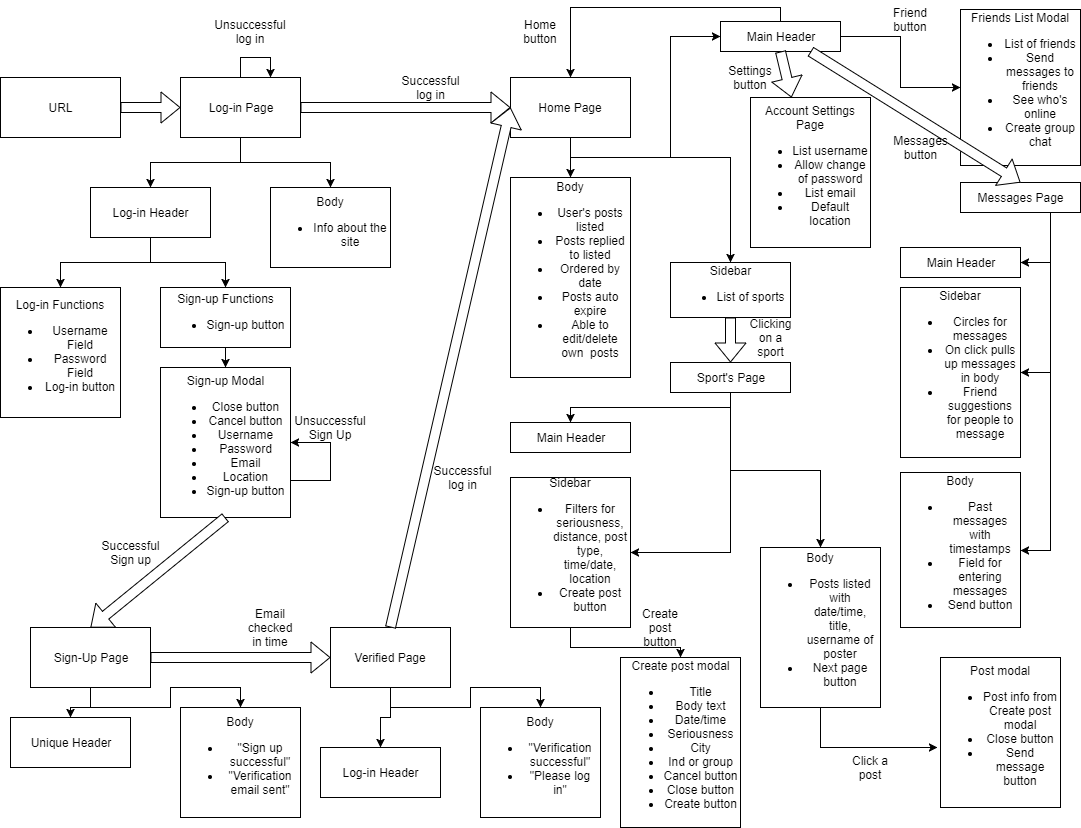
\includegraphics[width=1\textwidth]{cs361_1.png}
\newpage

\section{Packages}
There are several packages for our project: log-in page, home page, sports page, new event page, sign-up page, verification page, and a database. Their functions are written in Javascript.\\
\\
The log-in page is loosely coupled with every package; the user is required to log-in in order to create a new event or access the main details of the home page and home page. This allows the user's information to be stored onto a database, which an entry for the user's information is created through the sign-up page. The sign-up page is a key component of the log-in page, as the user is required to sign-up before using the website. The log-in page is otherwise independent of the rest of the packages.\\
\\
In addition, the log-in page is strongly cohesive. To be able to log-in, the user is required to sign-up on the sign-up page, which creates an entry on the database. After signing up, the user is required to verify their email to further modify the information stored on the database. There are several functions under logging in, such as validateLogin(), which checks if the user entered the correct log-in information and logs the user in, verifyEmail(), which indicates that the user is verified via a flag on the database, allowing them to access the rest of the website, errorMessage(), which indicates a bad log-in, and displaySport(), which displays the sports on the sports page if the user is verified.\\
\\
The homepage is loosely coupled with the rest of the packages as well. The homepage contains various functions that interact with the log-in page, sports page, new event page, sign-up page, and the database. The homepage displays all of the information stored on the database about events and has buttons that allows the user to access different aspects of the website. This only happens if the user is signed up and verified, but the homepage is otherwise independent.\\
\\
The homepage is also strongly cohesive. It allows the user to search the sports on the database using the function searchSports() and allows the user to apply filters to ease the search using applyFilters(). Afterwards, it will display the filtered results via displayResults(). The homepage also allows the user to create a new event by opening the new event modal after clicking on it. This function is known as onClick() and notifies the html to open up a new window. This window prompts the user to fill out the information about the event and creates the event via eventInfo() which pushes the data onto the database. Otherwise, it'll trigger the errorMessage() function which informs the user that their fields are incomplete.\\
\newpage


\section{Design Patterns}
The design pattern that we choose for our project is observer pattern.\\
\\
The observer pattern Defines a one-to-many dependency between objects so that when one object changes state, all its dependents are notified and updated automatically (1). In order to explain the reason why we use observer as our design pattern, I divide the definition of observer patter into two parts and compare these two parts with our project.\\
\\
\textbf{One-to-many dependency between objects.}\\
In the search function, every time the user chooses or types in a specific requirement in the filter, there are always a lot of available posts match the requirement. One filter requirement causes the multiple result posts.\\
\\
In the post event function, every time the user adds an event, all the information element of this event will be updated to the database, such as “post-title”, “post-location”, “post-date”. Adding one event causes the multiple element adding in database.\\
\\
\textbf{One object changes state, all its dependents are notified and updated automatically.}\\
In the search event function, once the user changes the information in the filter, the system will go through all the available posts in the database and update the “Post Result” part with the posts match the given filter information and display them in “Post Result” part.\\ 
\\
In the post event function, the system will store and detect all the information given by the user, and update and database with this new event. Taking a simple example to make things clearly.
Title: Come and join our basketball team
Date: Feb 10th, 2018
Seriousness: Medium
After adding this event, in the database, the “post-title” add one more element called “Come and join our basketball team”, the “post-date” add one more element called “Feb 10th, 2018”, the “post-seriousness” add one more element with the option of “Medium”. The latter two “post-date” and “post-seriousness” are attached to the “post-title”. So if the user searches the event with medium seriousness, then the “Come and join our basketball team” will show in the result posts.\\
\\
All in all, 
In the search page function, the filter part can be considered as an observer and the result post part is observed. Once some changes happen in filter, the post result will be updated by the changes.\\
In the post event function, the user interface can be considered as an observer and the database is observed. Once an event added (adding information by the pop-up windows), the database will be updated by adding all the information elements.

\newpage

\section{Interfaces and Contract}

For the website Pick Up, instances are being determined by the server actions as the HTML front-end is just an interface for the user to access the actions of the server.
 For much of the information coming out of these interfaces as postconditions, these are primarily being sent to a database internally that all interfaces have access to.
 The interfaces for the system are Log-In/Create Account, Home Page, Search, Create Post, and Messages. Each interface is detailed below.
\begin{wrapfigure}{r}{0.33\textwidth}
   \centering
   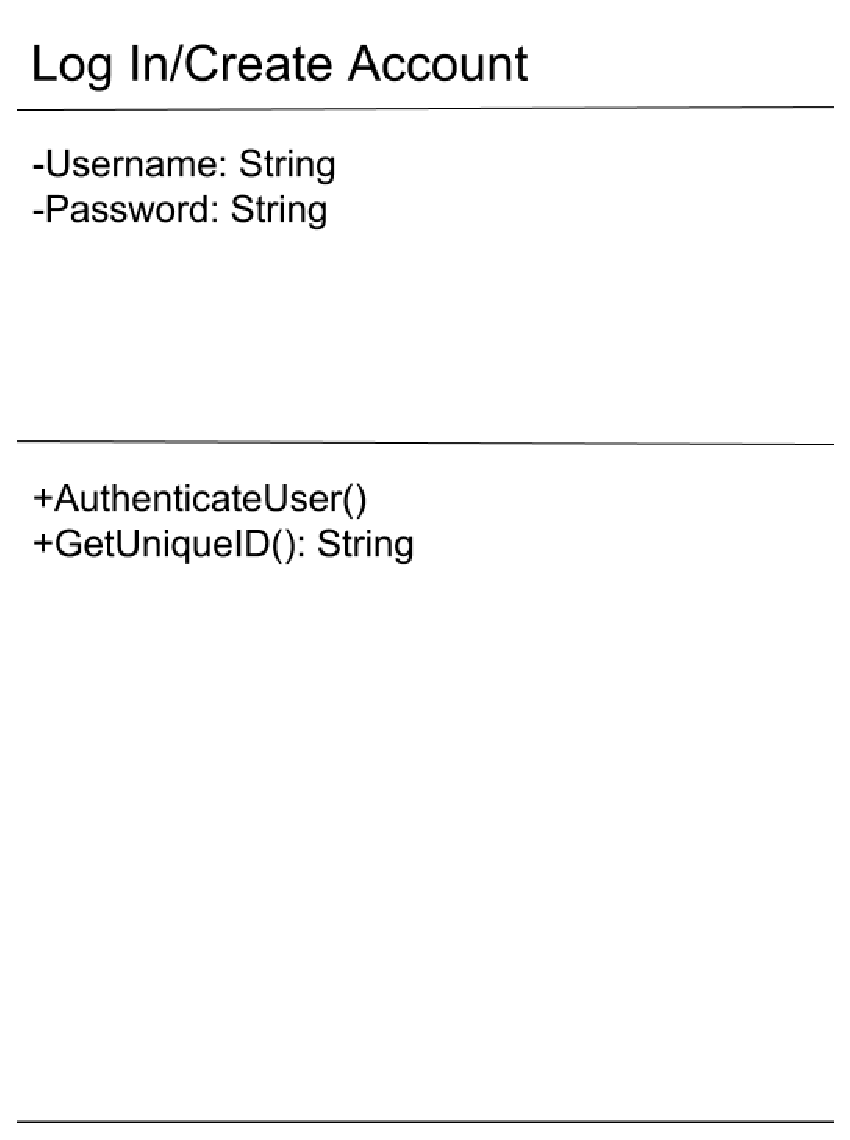
\includegraphics[width=0.33\textwidth]{LogIn.eps}
\end{wrapfigure}\\
\\
The Log-In/Create Account Interface is the first one experienced by the user and takes an input from the user of an account username and password. 
Since the username and password of the account are not supplied before this interface, they are not preconditions for the interface. 
The interface then returns a unique ID for the user log-in session. 
The Log-In and Create Account actions are combined in this Interface as both result in logging the user in with a unique ID that is directly passed to the next interface. 
Each action requires different information internally to either check with the database or add to the database, but the end result of logging a user in is the same.\\
\\
\begin{wrapfigure}{L}{0.33\textwidth}
   \centering
   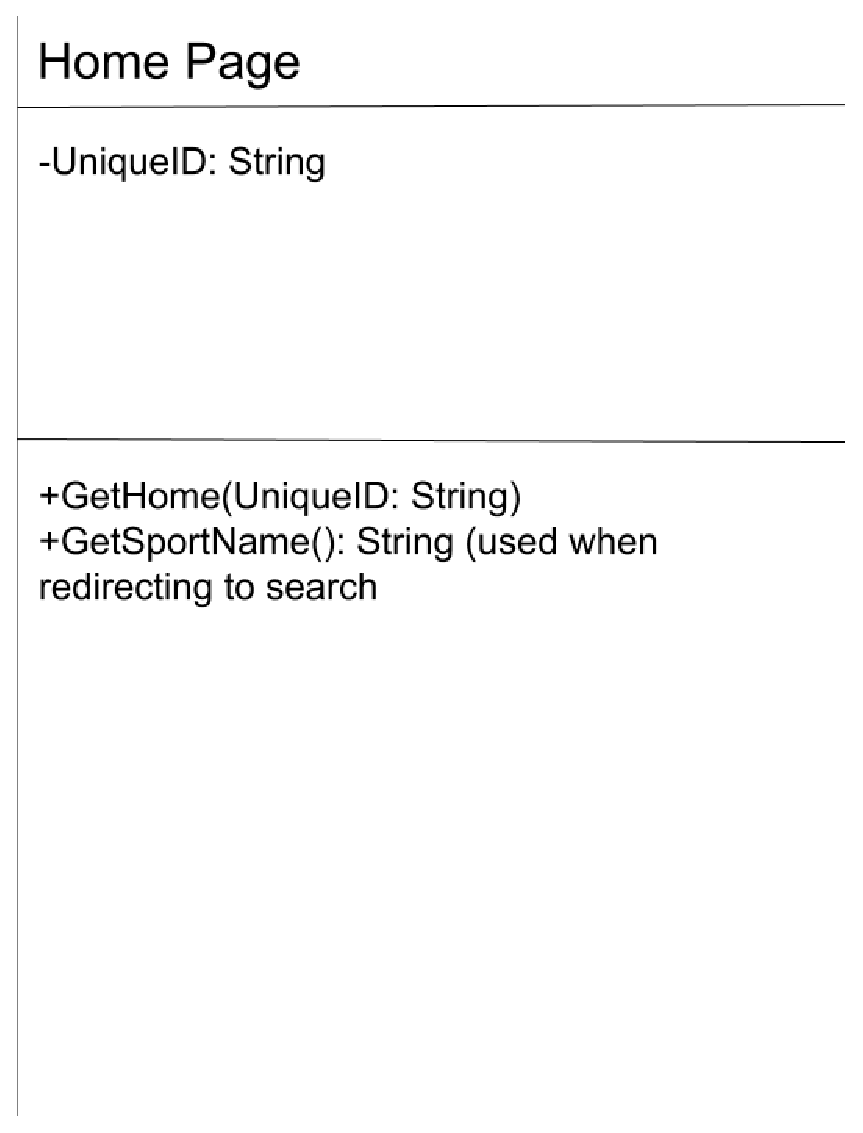
\includegraphics[width=0.33\textwidth]{HomePage.eps}
\end{wrapfigure}

The Home Page interface is accessed directly after the log-in interface and has the precondition of the unique ID from the log-in interface.  
The post-conditions of this interface is that the user will see listings from the database of events that the user is involved in. 
From the Home Page interface we can access two interfaces, the Messages interface and the Search interface. 
\clearpage
\begin{wrapfigure}{L}{0.33\textwidth}
   \centering
   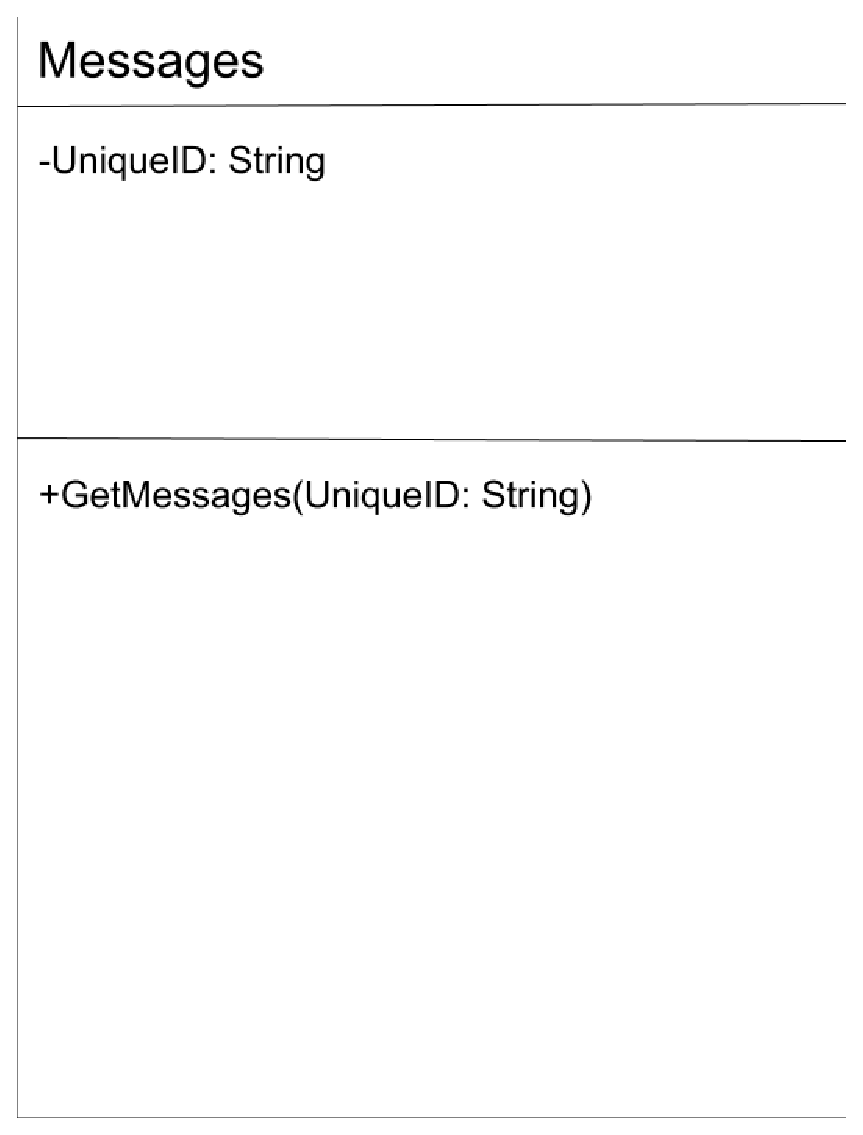
\includegraphics[width=0.33\textwidth]{Messages.eps}
\end{wrapfigure}

If the Messages interface is accessed, the Home Page sends the unique ID from log-in. 
If the Search interface is accessed, the Home Page sends the unique ID as well as the Sport Name that was selected by the user.

The Messages interface has the precondition of the unique ID of the user. 
The postconditions are each message from the database of that user to be displayed. 
This interface has no other interfaces attached to it.\\
\\\\\\\\\\\\\\
\begin{wrapfigure}{R}{0.33\textwidth}
   \centering
   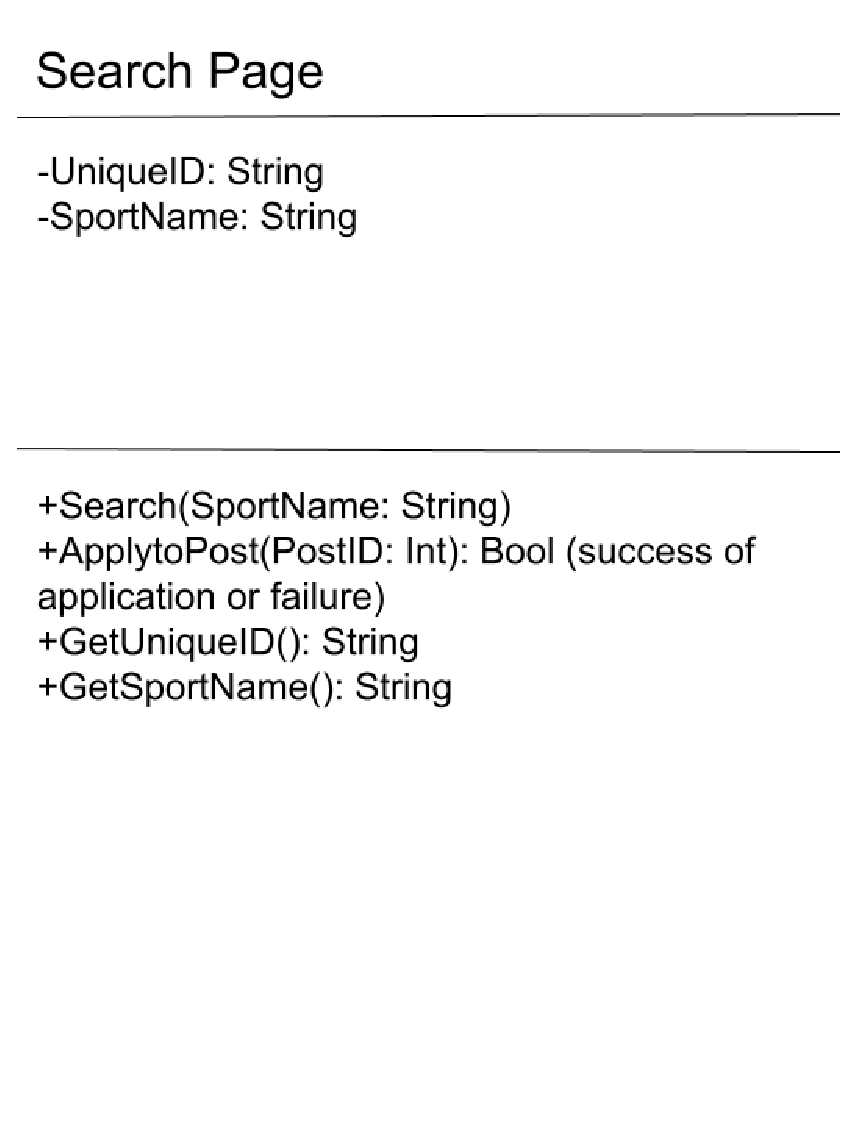
\includegraphics[width=0.33\textwidth]{SearchPage.eps}
\end{wrapfigure}

The Search interface has the preconditions of the unique ID of the user and the Sport Name that is to be searched. 
All searches for posts, regardless of the sport are treated the same way. 
The postconditions of this interface is the display of all created posts in the database that have a matching Sport Name to the one given to the Search interface. 
From here the Search interface can be called again with changed search conditions and the Create Post interface can also be accessed. 
If the Create Post interface is accessed, the Search interface will pass the unique ID of the user and the Sport Name to it as well. \\
\\\\\\\\\\
\begin{wrapfigure}{L}{0.33\textwidth}
   \centering
   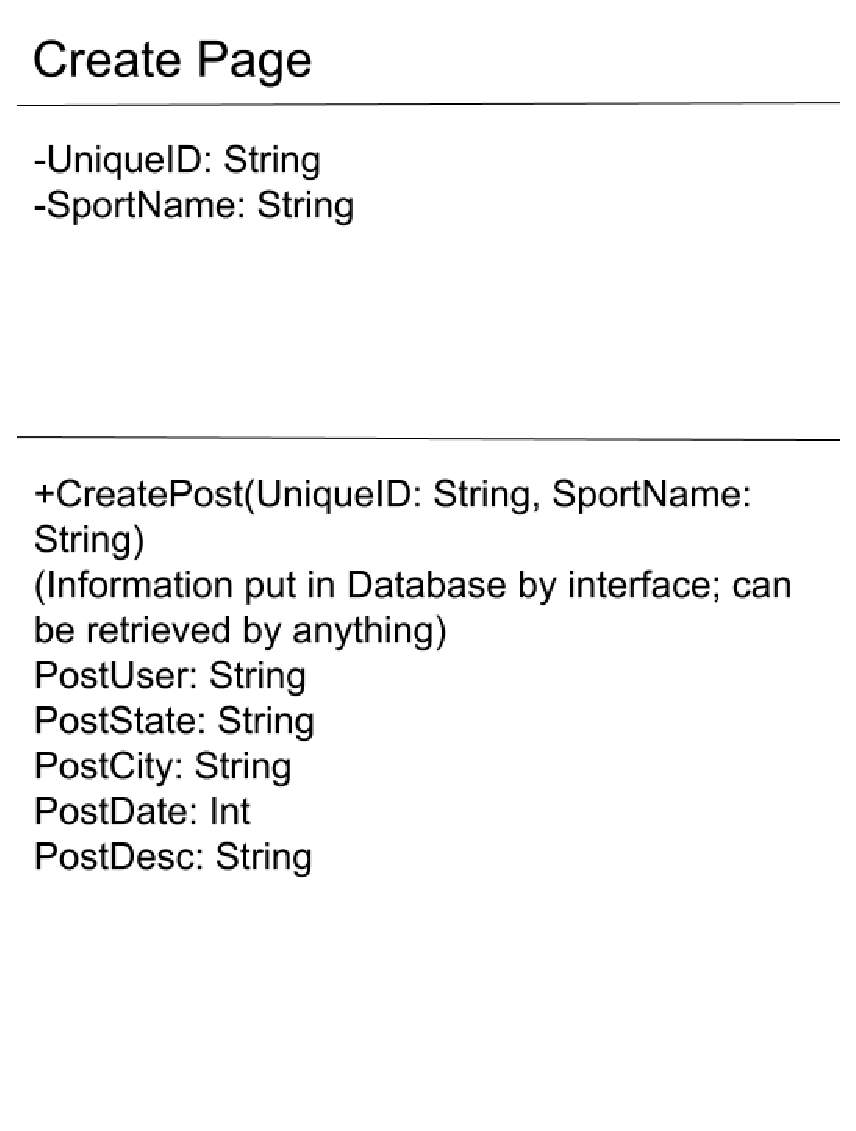
\includegraphics[width=0.33\textwidth]{CreatePost.eps}
\end{wrapfigure}

The Create Post interface has the preconditions of the unique ID of the user and the Sport Name that is to be searched. 
This is the final interface in the server design. 
The postconditions of this interface is the return of an HTML page with an HTML form for the user to enter details of the event they would like to create. 
Since this action can be cancelled, the actual creation of the event in the database is not a postcondition of the interface. 
From here we can cancel or submit the creation of a post but both return to the Search interface. 
With the submit action, the data entered in the form, if no errors appear, is written to the database.

\clearpage
\section{Exceptions \& Handling}
	One exception that may occur is bad input. We’ve classified bad input as any input that is invalid. This would occur in sign-up, log-in, and post creation. Causes we’ve identified would be entering a date that has already passed, entering invalid characters, entering inappropriate usernames, and others. We plan to handle this using regular expressions to verify strings and keeping track of the date in our JavaScript to make sure an invalid date hasn’t been entered. The user would receive an error message that pops up on screen along with the invalid field being cleared.\\
    \\
	Another exception we identified is nonexistent database entry. This would occur if a user tried to message or add another user, access a post that was deleted, or access a group that has been disbanded. Simply, if the user attempts to access something that doesn’t exist, this exception should be thrown. We can handle this by returning false if the function parsing through our database fails to find the requested information. In the case of a user attempting to message or add another user, an error message would pop up and the site would remain the same. If a user tried to access a nonexistent post, the page would refresh, clearing the deleted post, and an error message would be displayed. If the user tries to access a nonexistent group, an error message would be displayed.\\
    \\
	A third exception we thought of is expired verification. This would occur only when the email verification link has expired. If a user tries to verify their email past the allotted time, this exception will be thrown. The user should be redirected to a different page stating that the link expired and they must sign up again.\\
    \\
	Finally, we have a not found exception for all nonexistent URLs. This should bring the user to a 404 page and leave it at that.
    
\section{Meeting Report}
This week the group meet at 11:00 am in the Library on Friday, February 9th to
discuss assignment four, design and Implementation of your System (DIS). During this
meeting, we disused the requirements for the assignment to make sure everyone was
on the same page and then spit up the assignment into different parts for different group
members to work on. The assignment was split up so that Ryan will do the UML class
diagram and exceptions \&; handling sections, Cooper will do the Interfaces and Contract
section, Ziyu will do the design patterns section, Michael will do the packages section,
and Jordan will do the meeting report section. After discussing this week’s assignment
and the plan for progress, the meet ended at 12:00 pm with a plan to meet again on
Monday, February 12th at 4:00 pm to make the presentation as a group.\\
\\
The second meeting of this week took place at 4:00 pm in the Library on Monday
Friday, February 12th. At the meeting, the group worked on the presentation. First, the
team looked through the presentation requirements and discussed the basic format of
the presentation. While the group discussed this Ryan make the headings to of each of
the slides as discussed including requirements, purpose, major features, design, design
patterns, exceptions, planning, tasks, and risks. Then going back, we added pictures to
the as presentation based off of previously made diagrams and graphics. After that.,
collectively the group filled out the information for each slide and then split up the
presentation. Cooper will present slides 1-5. Ziyu will present slide six on design
patterns. Michael is going to present slide seven on package system. Ryan will present
the Class diagram on slide eight. Michael will present the Class diagram on slide nine.
UI will be presented by Ziyu on slide ten. Jordan will present sequence diagram on slide
eleven. Ryan will present slides 12-15. Finally, Cooper will finish the presentation with
slides sixteen and seventeen on risks. At 6:00 pm the meeting ended with a clear plan
for the presentation and everyone’s contributions.\\
\\
For next week, the group plans to meet 30 minutes before class on Tuesday,
February 13th to go over the presentation a few more times for practice so that
everyone in the group is clear and ready to present.

\end{document}